%!TEX root = ../thesis_a4.tex

\chapter{Automatic Construction of Music Knowledge Bases}
\label{sec:kb}

\section{Introduction}\label{sec:kb:introduction}

In this chapter, we present and evaluate an Information Extraction pipeline aimed at the construction of a Music Knowledge Base (\textsc{MKB}) entirely from scratch in an automatic and unsupervised manner.
We combine a state-of-the-art Entity Linking tool and a linguistically motivated rule-based algorithm to extract semantic relations between entity pairs. 
Our method is able to generate a fully disambiguated \textsc{MKB} with entity mappings against \textsc{DBpedia} and \textsc{MusicBrainz}. All relations have a relation pattern derived from a Relation Extraction (\textsc{RE}) procedure backed up by an algorithm that performs the following steps: (1) Morpho-syntactic rule-based \textit{filtering}; (2) Syntactic dependency-based \textit{clustering}; and (3) Relation \textit{weighting} based on statistical evidence. 

We validated our methodology on a large collection of documents in the music domain, obtained from \textit{songfacts.com}, a website that collects ``tidbits'' (short stories) about songs.
We carried out an intrinsect evaluation on each component of the algorithm, as well as an extrinsic evaluation which consists of a experiment on interpretation of music recommendations, where our automatically learned \textsc{MKB} is used to provide explanations to song recommendations in \textit{natural language}.
Our experimental results indicate that our system is able to extract \textit{high quality} relations (Precision $>= 0.8$) as well as \textit{novel knowledge}. We unveil thousands of relations absent in both large-scale generic \textsc{KBs}, as well as in music specific resources. Moreover, the recommendation explanation experiment shows that explanations based on the newly learned \textsc{KB} have a positive impact in user experience.

%We release the learned \textsc{MKB} at several confidence levels, together with the evaluation data used in the experiments described in this chapter. The code for the complete \textsc{RE} pipeline is also released as open source software under MIT license.

The main contributions of this chapter are summarized as follows:
\begin{itemize}
    \item{We address for the fist time the problem of automatic construction of MKBs from plain text.}
    \item{We put forward a novel approach for clustering relations, based on patterns derived from syntactic dependencies.}
    \item{We present a new confidence measure over all extracted relations and demonstrate its discriminative power.}
    \item{We showcase the utility of our method by creating a high quality MKB with \textit{novel knowledge}.}
    \item{We demonstrate the usefulness of our automatically constructed MKB for providing explanations in natural language in the context of music recommendation.}
\end{itemize}

The work described in this chapter is a joint effort by the author of this thesis, and Luis Espinosa-Anke, both researchers in the UPF Department of Information Technologies. This collaboration is framed within the Maria de Maeztu strategic program, specifically in the Music Meets NLP project.

The rest of this chapter is organized as follows. In Section~\ref{sec:kb:method} we describe step by step the proposed methodology for relation extraction. Then, in Section~\ref{sec:kb:exp} we illustrate the gathered dataset and the outcome of the relation extraction process. The results of our evaluation are reported in Section~\ref{sec:kb:experiments}, and the chapter ends with a discussion about our findings and future work.


\section{Method}
\label{sec:kb:method}

We propose a comprehensive pipeline that learns a full-fledged \textsc{MKB} taking as input raw text collections. The experiments we report in this chapter are the result of applying our method to a dataset of plain text extracted from the Songfacts\footnote{\url{http://www.songfacts.com}} website (see Section~\ref{sec:kb:exp:dataset}). This is a well suited resource both for \textsc{KB} learning and as a testebed for \textsc{RE} due to its specificity. Essentially, Songfacts documents, while not being as rigid as encyclopedic text or newswire text, remain well-formed, sentences make sense, and there is no need for \textit{ad-hoc} preprocessing (as it is required in social networks, e.g. Twitter). Our method, however, can be ported with little effort to music-related corpora of different registers.

\subsection{Notation}

Our method focuses on the extraction of semantic relations between pairs of  linked entities (e.g. \textit{Born in the USA}$_{dbr}$, \textit{Bruce Springsteen}$_{dbr}$\footnote{We use the \textit{dbr} subscript to refer to disambiguated entities linked to \textsc{DBpedia} resources.}), which are in turn associated to specific entity types (e.g. \textit{Album}, \textit{MusicalArtist}). In our \textsc{KB}, a relation $r$ is defined by the tuple $\langle \textbf{\textit{e}}{_\textbf{\textit{d}}},
\textbf{\textit{e}}{_\textbf{\textit{r}}},
\boldsymbol\upsilon{_\textbf{\textit{d}}},
\boldsymbol\upsilon{_\textbf{\textit{r}}},
\textbf{\textit{p}}, \textbf{\textit{c}}\rangle$, where \textbf{\textit{d}} and \textbf{\textit{r}} refer to domain and range positions, $\textbf{\textit{e}}{_\textbf{\textit{d}}}$ and $\textbf{\textit{e}}{_\textbf{\textit{r}}}$ to the entities involved in the relation, $\boldsymbol\upsilon{_\textbf{\textit{d}}}$ and
$\boldsymbol\upsilon{_\textbf{\textit{r}}}$ to their associated entity types, \textbf{\textit{p}} to a relation pattern, and \textbf{\textit{c}} to a cluster pattern.  
A relation pattern is a relation label that may be used in one or several relations (e.g \textit{was recorded by frontman}, \textit{was recorded by singer/songwriter}). Relation patterns with similar semantic and syntactic characteristics may be grouped into cluster patterns (e.g. \textit{was recorded by}). 
$\mathcal{R}$ denotes the set of all extracted relations included in the \textsc{KB}.
For each $r \in \mathcal{R}$, triples of different nature can be constructed by arbitrarily combining elements in $r$.

\begin{itemize}
    \item $t_\textbf{\textit{p}}: \langle \textbf{\textit{e}}{_\textbf{\textit{d}}},\textbf{\textit{p}},\textbf{\textit{e}}{_\textbf{\textit{r}}} \rangle$ , e.g. \{\textit{Born in the USA}$_{dbr}$ - \textit{was recorded by frontman} - \textit{Bruce Springsteen}$_{dbr}$\}.
    \item $t_\textbf{\textit{c}}: \langle \textbf{\textit{e}}{_\textbf{\textit{d}}},\textbf{\textit{c}},\textbf{\textit{e}}{_\textbf{\textit{r}}} \rangle$ , e.g. \{\textit{Born in the USA}$_{dbr}$ - \textit{was recorded by} - \textit{Bruce Springsteen}$_{dbr}$\}.
    \item $\tau_\textbf{\textit{p}}: \langle \boldsymbol\upsilon{_\textbf{\textit{d}}},\textbf{\textit{p}},\boldsymbol\upsilon{_\textbf{\textit{r}}} \rangle$ , e.g. \{\textit{Album} - \textit{was recorded by frontman} - \textit{MusicalArtist}\}.
    \item $\tau_\textbf{\textit{c}}: \langle \boldsymbol\upsilon{_\textbf{\textit{d}}},\textbf{\textit{c}},\boldsymbol\upsilon{_\textbf{\textit{r}}} \rangle$ , e.g. \{\textit{Album} - \textit{was recorded by} - \textit{MusicalArtist}\}.
\end{itemize}

Finally, different subsets of $\mathcal{R}$ may be constructed by selectively filtering all $r \in \mathcal{R}$.  

\begin{itemize}
    \item $\mathcal{R}_{p} = \{r_1^p, ... r_n^p\}$ All relations with a specific relation pattern $p$.
    \item $\mathcal{R}_{c} = \{r_1^c, ... r_n^c\}$ All relations with a specific cluster pattern $c$.
    \item $\mathcal{R}_{\boldsymbol\tau{_\textbf{\textit{p}}}} = \{r_1^{\tau{_p}}, ... r_n^{\tau{_p}}\}$ All relations with a specific relation pattern, and domain and range entity types.
    \item $\mathcal{R}_{\boldsymbol\tau{_\textbf{\textit{c}}}} = \{r_1^{\tau{_c}}, ... r_n^{\tau{_c}}\}$ All relations with a specific cluster pattern, and domain and range entity types.
\end{itemize}

In what follows, we describe a method for acquiring new entities, types and relations, and combining them in a meaningful way for \textsc{KB} construction.


\subsection{Morphosyntactic Preprocessing}\label{sec:kb:method:preprocessing}

Our morphosyntactic preprocessing module takes as input a collection of text documents in the music domain. First, sentence splitting and tokenization is carried out thanks to the \textit{Stanford NLP tokenizer}\footnote{\url{http://nlp.stanford.edu/software/tokenizer.shtml}}. 
Next, a dependency parse tree is obtained via the MATE Parser, described in \cite{Bohnet2010}. We justify the use of the latter because of the richness of its tagset, as well as performance in terms of accuracy and speed, which were appropriate for the task at hand.

In a dependency tree, each node includes information, at least and depending of the model and the language, about surface and lemmatized forms, along with its part-of-speech. Each edge in the tree is labeled with a dependency relation such as \textit{subject} or \textit{noun modifier} (an example is shown in Figure ~\ref{fig:kb:sampletree}).


\begin{figure}[!htb]
\centering
\begin{dependency}
\begin{deptext}[column sep=.0cm]
NN \& NN \& VBD \& VBN \& IN \& NNP \& NNP \\
\textbf{Sweet} \& \textbf{Freedom} \& was \& written \& by \& \textbf{Rod} \& \textbf{Temperton} \\
\end{deptext}

\deproot[edge height=10ex]{3}{root}

\depedge[edge style={ultra thick, dotted}]{3}{2}{SBJ}
\depedge[edge style={ultra thick, dotted}]{3}{4}{VC}
\depedge[edge style={ultra thick, dotted}]{2}{1}{NAME}

\depedge[edge style={ultra thick, dotted}]{4}{5}{LGS}
\depedge[edge style={ultra thick, dotted}]{5}{7}{PMOD}
\depedge[edge style={ultra thick, dotted}]{7}{6}{NMOD}

\end{dependency}
\vspace*{-5mm}
\caption{Example sentence with dependency parsing tree}
\label{fig:kb:sampletree}
\end{figure}


\subsection{Semantic Processing: Entity Linking}
\label{sec:kb:method:entitylinking}

Entity Linking (\textsc{EL}) acts as a semantic bridge between plain text and a reference knowledge inventory. While there are a number of popular \textsc{EL} systems which are not bound to any domain or discipline, there is no benchmark of such systems in the music domain. Therefore, we do not know \textit{a priori} how well each of them works in music corpora. Musical entities may raise a plethora of challenges, derived mostly from ambiguity and polysemy. For example, an album may have the same name as the band who recorded it (e.g. \textit{Weezer} the band and their first album). Moreover, an artist, a song or an album may have words or expressions much more common in another domain or area of knowledge (e.g. \textit{Berlin, The Who}). Thus, the choice of the best \textsc{EL} algorithm or off-the-shelf tool(s) is crucial, as potential errors may propagate throughout the different modules and hinder considerably the quality of the resulting \textsc{KB}.

Among the available EL systems we considered, namely \textsc{Tagme} \cite{Ferraginaetal2010}, \textsc{Babelfy} \cite{Moroetal2014} and \textsc{DBpedia} Spotlight \cite{Mendes2011}, we opted for the latter, as it has shown to be the least prone to errors in musical texts (further details are provided in Section~\ref{sec:kb:experiments:qualityentitylinking}).

\subsubsection{Adding Co-references}

In the music domain, prototypical factoid documents such as artist biographies, album reviews, or song tidbits, normally refer to one specific entity. Based on this observation, we may exploit co-referential pronouns and \textit{resource-specific co-references}, replacing them by the name of the reported entity.
A similar approach is used in \cite{Voskarides2015}, where the frequency of pronouns ``he'' and ``she'' is computed in every document (Wikipedia articles in this specific case) to determine the entity's gender, and then, these pronouns are replaced by the entity title. %Similarly, in \cite{Oramas2014}, a gender identifier web service is used to determine the gender of subjects in artist biographies as part of a \textsc{RE} pipeline.

We have observed an exploitable \textit{resource-specific co-reference} in music reviews, where terms like ``this album'' or ``the song'' can be replaced by the document's title. In the dataset used for the experiments (see Section~\ref{sec:kb:exp:dataset}), the expressions ``this song'' and ``the song'' are replaced with the name of the song as it appears in the document, and disambiguated with the URI of the entity they unequivocally refer to.

Co-reference resolution is a difficult and crucial task in NLP, affecting tasks such as Information Extraction \cite{Soon2001} or document summarization \cite{saggion2004multi}. It is also sensitive to the domain in which it appears (see, for instance, the case of the patents domain \cite{Bouayad2014}). We acknolwedge the difficulty of this task. However, while addressing this problem in its entirety is out of the scope of this chapter, these strategies allow us to increase coverage of entity mentions while maintaining a high precision.



\subsubsection{Type Filtering}
\label{sec:kb:typefiltering}

In \textsc{DBpedia}, most resources are associated with one or more types via the \texttt{rdf:type} property. In addition, among the different types present in \textsc{DBpedia} (coming from the \textsc{DBpedia} ontology, \textsc{Yago} types, or \texttt{schema.org}), the \textsc{DBpedia} ontology provides a relatively small and tidy taxonomy of 685 classes based on \textsc{Wikipedia} infoboxes. Other \textsc{KBs} such as \textsc{Yago} or Freebase have their own ontological structure, which is in general broader and noisier. \textsc{MusicBrainz}, in contrast, has a very narrow set of entity types. 

This type information can be exploited in order to narrow down the set of allowed types for a given candidate and its potential annotations. In this way, we ensure that all entities will be, at least, related to the music domain. Restricting the search space to types such as Artist or Song reduces considerably the number of errors derived from cross-domain ambiguity. For instance, the EL system detects a substantial amount of entities whose DBpedia type is \textit{FictionalCharacter}, which are in most of the cases misleading song titles or band names with fictional characters of the same name. This situation is observed also with other types of entities such as \textit{Athlete}, \textit{Species} or \textit{Disease}.

Depending on the envisioned application of the \textsc{KB} resulting from our pipeline, the predefined set of entity types may vary. In our case we restricted them to Musical Artists, Other Artists, Songs, Albums, Genres, Films and Record Labels. In Table~\ref{tbl:kb:type_mapping} we present the mapping between the \textsc{DBpedia} ontology, \textsc{MusicBrainz} entity types and our selected set of types.

\begin{table*}[ht!]
\scriptsize
\centering
	\begin{tabular}{ | l | l | l | }
	\hline
\textbf{Our \textsc{MKB}} & \textbf{\textsc{DBpedia} ontology} & \textbf{\textsc{MusicBrainz}} \\
	\hline
\multirow{4}{*}{MusicalArtist} & Person/Artist/MusicalArtist & \multirow{4}{*}{Artist}\\ 
& Organization/Band & \\ 
& Writer/MusicComposer & \\ 
& Writer/SongWriter & \\
	\hline
\multirow{2}{*}{OtherArtist} & Person/Artist ($\neg$ MusicalArtist) & \multirow{2}{*}{---} \\
& Person/Writer($\neg$ MusicComposer \& $\neg$ SongWriter) & \\
    \hline
Album & Work/MusicalWork/Album & Release \\
    \hline
\multirow{2}{*}{Song} & Work/MusicalWork/Song & Recording \\
& Work/MusicalWork/Single & Work \\
    \hline
Genre & TopicalConcept/Genre & --- \\
    \hline
Film & Work/Film & --- \\
    \hline
RecordLabel & Agent/Organization/Company/RecordLabel & Label \\
    \hline
	\end{tabular}
	\caption{Type mapping.}
	\label{tbl:kb:type_mapping}
\end{table*}
%

\subsection{Syntactic Semantic Integration}
\label{sec:kb:method:syntsemint}

The information obtained from the syntactic and semantic processes is combined into a graph representation of the sentence. For each music entity identified during the semantic enrichment step (Section~\ref{sec:kb:method:entitylinking}), all nodes in the dependency tree with a correspondence with an entity mention are collapsed into one single node: \textit{Sweet} and \textit{Freedom} into \textit{Seet Freedom (Album)}, and \textit{Rod} and \textit{Temperton} into \textit{Rod Temperton (Artist)}. Figure ~\ref{fig:kb:sampletree_combined} shows the resulting syntactic-semantic representation of a sentence.

\begin{figure}[!htb]
\centering
\begin{dependency}
\begin{deptext}[column sep=.0cm]
\textbf{Album} \& VBD \& VBN \& IN \& \textbf{Person} \\
\textbf{Sweet Freedom} \& was \& written \& by \& \textbf{Rod Temperton} \\
\end{deptext}

\deproot[edge height=10ex]{4}{root}

\depedge[edge style={ultra thick, dotted}]{2}{1}{SBJ}
\depedge[edge style={ultra thick, dotted}]{2}{3}{VC}
\depedge[edge style={ultra thick, dotted}]{3}{4}{LGS}
\depedge[edge style={ultra thick, dotted}]{4}{5}{PMOD}

\end{dependency}
\vspace*{-5mm}
\caption{Semantic integration on syntactic dependencies.}
\label{fig:kb:sampletree_combined}
\end{figure}


\subsection{Relation Extraction and Filtering}
\label{sec:kb:method:re-filtering}

Our approach to RE is lightweight, unsupervised and rule-based. Having syntactic and semantic information available, potential relations between entities may be discovered by traversing the dependency tree.
Two entities in such tree are considered to be related if there is a path between them that does not contain any other entity in between, and does not contain parentheses. If there is more than one path, we consider only the shortest path as the most representative path of the relation.

Our method encodes a relation pattern between two entities as all words in the shortest path between them. In the example provided in Figure ~\ref{fig:kb:sampletree_combined}, the shortest path between \emph{Sweet Freedom} and \emph{Rod Temperton} contains the words \textit{was}, \textit{written} and \textit{by}.

While RE via shortest path in syntactic trees is common practice in the literature \cite{DelliBovietal2015b,MoroandNavigli2012,Nakasholeetal2012}, not all shortest paths are valid, and incorrect relations may be extracted from overly long and syntactically complex sentences. We aim at surmounting these problems by defining three filtering heuristics over surface forms (\textit{lemma-paths}), part-of-speach patterns (\textit{pos-paths}), and labels of syntactic dependencies (\textit{dependency-paths}).

First, we filter out all relations with reporting verbs (e.g. ``say'', ``tell'' or ``express'') in the lemma-path. The intuition being that sentences with these verbs are by definition syntactically complex, and semantic relations in them may not be encoded via shortest paths. We illustrate this with the following sample sentence, where the relation extracted with syntactic tree traversal by means of shortest path would be incorrect:

\begin{itemize}
\item[] \textbf{Sentence:} \texttt{Nile Rodgers} \textit{told} NME that the first album he bought was Impressions by \texttt{John Coltrane}.
\item[] \textbf{Relation}: \texttt{nile\_rodgers} told that was impressions by \texttt{john\_coltrane}
\end{itemize}

Second, we only selected relations where the syntactic function that connects in the dependency-path the fist entity with the first word of the relation pattern is a subject (which may be preceded by a nominal modifier or an apposition), a direct or indirect object, a predicative complement or a verb chain. When this condition holds, the relation is considered \textit{valid}. If the above condition does not hold, an extra validation step is applied over the pos-path in order to capture relations without verbs, which seem to be idiosyncratic of the music domain, e.g. $\langle e_d, \mbox{\texttt{frontman of}}, e_r \rangle$, $\langle e_d, \mbox{\texttt{drummer}}, e_r \rangle$, or $\langle e_d, \mbox{\texttt{guitarist and singer}}, e_r \rangle$.

\subsection{Dependency-Based Loose Clustering}
\label{sec:kb:method:clustering}

In this section we describe a simple but powerful clustering algorithm aimed at reducing the number of relation patterns in the \textsc{KB}. %noise in our relation patterns inventory.% inventory $\mathcal{P}$.

Let us consider the following three relation patterns: (1) \textit{was written by blunt producer}, (2) \textit{was written by singer/producer}, and (3) \textit{was written by manager and guitarist}. Intuitively, these three relation patterns seem to be semantically similar, and if all of them were expressed as \textit{was written by}, the original meaning would not be lost, and the set of relations would become more compact.

This observation, which we found to occur quite frequently, motivated the inclusion of a \textit{dependency-based loose clustering} module. First, we perform a second run of dependency parsing over all relation patterns extracted by our system, aiming at discovering their root node. We apply this second run because the root of the original sentence does not need to correspond with the relation pattern's root. Then, our algorithm considers all possible paths from the root to every leaf node of the relation pattern dependency tree, and selects the path that complies with a predefined syntactic constraint (e.g. a sequence of verbs plus adverb or preposition, or adverb plus nominal and preposition modifiers) based on regular expressions of syntactic labels. The sequence of tokens that matches this regular expression constitutes the cluster pattern. The complete set of defined regular expressions is included in the released source code.

As an illustrative case, consider the extracted relation pattern \textit{is track was released on label} from the sentence \textit{\texttt{Sing Out The Song} is the 7th track on Wishbone Four which was released in the UK May 1973 on the \texttt{MCA} label}. After re-parsing the relation pattern, we obtain the parse tree shown in Figure \ref{fig:kb:parsedpattern} and a cluster pattern over those nodes in the dependency tree that satisfy one of the regular expressions crafted in the aforementioned syntactic constraint. Finally, the obtained relation is \textit{\texttt{Sing\_out\_the\_song} was released on label \texttt{MCA}}.

\begin{figure}[!htb]
\centering
\begin{dependency}
\begin{deptext}[column sep=.5cm]
is \& track \& was \& released \& on \& label \\
\end{deptext}

\deproot[edge height=10ex]{3}{root}

\depedge[edge style={}]{3}{2}{SBJ}
\depedge[edge style={ultra thick}]{3}{4}{VC}
\depedge[edge style={}]{2}{1}{NMOD}

\depedge[edge style={ultra thick}]{4}{5}{ADV}
\depedge[edge style={ultra thick}]{5}{6}{PMOD}

\end{dependency}
\vspace*{-5mm}
\caption{Example of a parsed relation pattern $p \in \mathcal{P}$ and a valid cluster pattern (bold).}
\label{fig:kb:parsedpattern}
\end{figure}


Filtering out spurious information in OIE following similar approaches has proven effective while not being computationally expensive \cite{Fader2011}.

Ours is a \textit{loose clustering} method because it does not enforce a pattern to fully match all rules, but rather allows partial matching. This module provides an enrichment of all $r \in \mathcal{R}$ such that $r = \langle e_d, e_r, \upsilon_d, \upsilon_r, p, c\rangle$, where $c$ is the cluster pattern derived from the relation pattern $p$. A relation cluster is the set of all relations with the same cluster pattern, and is denoted as $\mathcal{R}_c$. 


\begin{table*}[ht!]
\scriptsize
	\begin{tabular}{ | l | l | l | }
	\hline
\textbf{Cluster pattern $c$} & \textbf{Typed cluster pattern $ \tau_\textbf{\textit{c}}$} & \textbf{Relation triples $t_\textbf{\textit{p}}$} \\
\hline
\multirow{10}{*}{\textit{was written by}} & \multirow{3}{*}{S \textit{was written by} MA} & s1 \textit{was writen by artist} ma1 \\
\cline{3-3}
 &  & s2 \textit{was written by composer} ma2 \\
\cline{3-3}
 &  & s3 \textit{was written by singer} ma2 \\
\cline{3-3}
&  & s4 \textit{was writen by} ma1 \\
 \cline{3-3}
&  & s5 \textit{was written by frontman} ma3 \\
\cline{2-3}
& \multirow{3}{*}{A \textit{was written by} MA} & a1 \textit{was written by frontman} ma3 \\
 \cline{3-3}
&  & a2 \textit{was written by guitarist} ma1 \\
\cline{3-3}
&  & a3 \textit{was written by artist} ma2 \\
\cline{3-3}
&  & a4 \textit{was written by frontman} ma5 \\
    \hline
	\end{tabular}
	\caption{Example of a relation cluster $\mathcal{R}_c$, where $c = \mbox{\textit{was written by}}$. \textit{S} refers to Song, \textit{MA} to MusicalArtist and \textit{A} to Album types, whilst \textit{sX} refers to Song, \textit{maX} to MusicalArtist and \textit{aX} to Album entities.}
	\label{tbl:kb:example_grouping}
\end{table*}


\subsection{Scoring}
\label{sec:kb:method:scoring}

So far, our approach has identified entity mentions in text and has linked them in meaningful relations, filtering out those that did not comply with predefined linguistic rules. We incorporate one additional factor $score(r)$ that takes into account statistical evidence computed over $\mathcal{R}$. It has three main components, which we flesh out as follows.

We hypothesize that the relevance of a cluster may be inferred by the number and proportion of triples it encodes, and whether these are evenly distributed. 
Our metric encompasses a combination of three different components. First, we focus on the \textit{degree of specificity} of the relation cluster, as previous work has demonstrated that this can contribute to Information Extraction pipelines \cite{DelliBovietal2015}. Second, we analyze \textit{intrinsic features} of the relation pattern, such as frequency, length and fluency. Finally, we incorporate a \textit{smoothing factor}, namely the proportion of the related typed cluster pattern in the cluster.

A cluster $\mathcal{R}_c$ may be decomposed into a set of typed cluster patterns $\tau_c$ (see Table ~\ref{tbl:kb:example_grouping}). The intuition behind the specificity measure of a cluster is that clusters with one prominent $\tau_c$ are more specific, i.e. they are largely used for encoding one specific type of relations. One example of this would be \textit{performed with}, which enforces a relation to include MusicalArtists on both the domain and range sides. Thus, we define $\mathcal{L}_c$ as the list of cardinalities (number of triples) of every typed cluster pattern $\tau_c \in \mathcal{R}_c$, being $\mathcal{L}_c = \{|\mathcal{R}_{\tau_c^1}|,...,|\mathcal{R}_{\tau_c^n}|\}$. We define the specificity measure as the variance of $\mathcal{L}$, expressed as $s(\mathcal{R}_c) = var(\mathcal{L}_c)$.

Furthermore, we consider a \textit{relation's fluency} metric, which is aimed at capturing its comprehensibility. Simply put, the more the sentence's original word order is preserved in the relation pattern, the more understandable it should be. This metric is introduced due to the fact that word order is lost after modelling text under a dependency grammar framework, and so we design a \textit{penalty measure} over the number of jumps needed to reconstruct the original ordered word sequence. Let $k$ be the number of tokens in the relation pattern, $w_i$ the $ith$ word in the pattern, and $h(w_i)$ a function that returns the correspondent word index in the original sentence, we put forward a fluency measure $f$ defined as:

\begin{equation}
f(p) = \frac{\sum_{i=1}^{k} \alpha | h(w_i) - h(w_{i-1}) |}{k}
\end{equation}

where $\alpha=2$ if $h(w_{i-1}) > h(w_i)$ and $\alpha=1$ otherwise. Note that higher values of $f$ means low fluency. For instance, for the relation pattern \textit{is hit for} the score would be much higher than a mixed-up order relation pattern such as \textit{joined because added were and hit}, which would have a very high $f$.  

Finally, the global confidence measure for each relation $r \in R$ is expressed as follows:

\begin{equation}
score(r) = \left({s(\mathcal{R}_c) + \frac{|\mathcal{R}_p|}{|p|+2^{f(p)}}}\right) \times {\frac{|\mathcal{R}_{\tau_c}|}{|\mathcal{R}_c|}}
\end{equation}

As an illustrative example of the measure, the score of a relation with the typed cluster pattern $\langle$Song, \textit{was released on}, RecordLabel$\rangle$, will have a much higher score than a relation whose typed cluster pattern is $\langle$Album, \textit{was released on}, MusicalArtist$\rangle$. This latter pattern is incorrect, probably due to a disambiguation error in the \textsc{EL} step. Relations like this show the type of errors which our proposed confidence score is expected to consider for pruning.



\section{Experimental Setup}\label{sec:kb:exp}

In this section, we describe our experimental setting. We refer first to the source raw corpus, and second to the resulting \textsc{KBs} as output of different branches of our approach.


\subsection{Source dataset}\label{sec:kb:exp:dataset}

Songfacts\footnote{\url{http://www.songfacts.com}} is an online database that collects, stores and provides facts, stories and trivia about songs. These are collaboratively written by registered users, and reviewed by the website staff. It contains information about more than 30,000 songs from nearly 6,000 artists. This information may refer to what the song is about, who wrote it, who produced it, who collaborated with whom or who directed the video. These texts are rich sources of information not only for well-known music facts, but also for music-specific trivia, as in the following sample sentence (about David Bowie's \textit{Space Oddity}): ``Bowie wrote this song after seeing the 1968 Stanley Kubrick movie 2001: A Space Odyssey".

We crawled the Songfacts website in mid-January 2014. Then, for each song article, we performed a mapping between the song and its \textsc{MusicBrainz} song ID, using the \textsc{MusicBrainz} Search API. We successfully mapped 27,655 songs.

The \textsc{RE} pipeline was run over the 27,655 document Songfacts corpus, which amounts to 306,398 sentences. After the Semantic Processing step, we obtained 202,767 entity mentions (8,880 for \textit{Albums}, 3,136 \textit{Record Labels}, 74,908 \textit{Songs}, 107,253 \textit{Musical Artists}, 1,760 \textit{Genre} labels, 3,467 for \textit{Other Artist}, and 3,363 for \textit{Film}). There were 48,122 sentences with at least two entities, and it is on this subset where we apply our RE pipeline.


\subsection{Learned Knowledge Bases}
\label{sec:kb:exp:learnedkbs}

Our aim is to assess to what extent each of the modules integrating our approach contributes to the quality of the resulting \textsc{KB}. After executing the whole pipeline, we generate two \textit{learned} \textsc{KBs} (\textsc{KBSF}-ft and \textsc{KBSF}-th), two \textit{baseline} \textsc{KBs} (\textsc{KBSF}-co and \textsc{KBSF}-raw), and a \textit{competitor} \textsc{KB} (\textsc{KBSF}-rv). 

The \textit{learned} \textsc{KBs} are the result of applying the \textsc{RE} method to the Songfacts dataset under different conditions. \textsc{KBSF}-ft is derived from applying the \textsc{RE} pipeline entirely, and \textsc{KBSF}-th comes from a selection of all triples in \textsc{KBSF}-ft with a confidence score above a certain threshold. To determine the best threshold to prune \textsc{KBSF}-ft, we aimed at maximizing the number of triples and at the same time minimizing the number of relation patterns. Our intuition is that less patterns means a tidier \textsc{KB}. Therefore, we computed the percentage of triples and relation patterns from \textsc{KBSF}-ft that remain in a pruned \textsc{KB}, whose triples have a score greater than a certain threshold $\theta$. We computed these percentages for every $\theta$ value ranging from 0 to 1 in bins of 0.01 (see Figure \ref{fig:kb:th}). Our goal was to discover the $\theta$ value which maximizes the distance between the amount of triples and the amount of relation patterns in a pruned \textsc{KB}. After confirming a maximized difference with $\theta=0.05$, we created \textsc{KBSF}-th, whose triples have a score greater than or equal to 0.05. In this pruned \textsc{KB}, we have 36.56\% of \textsc{KBSF}-ft triples, with only 12.52\% of its relation patterns.

\begin{figure}[!htp]
\centerline{\framebox{
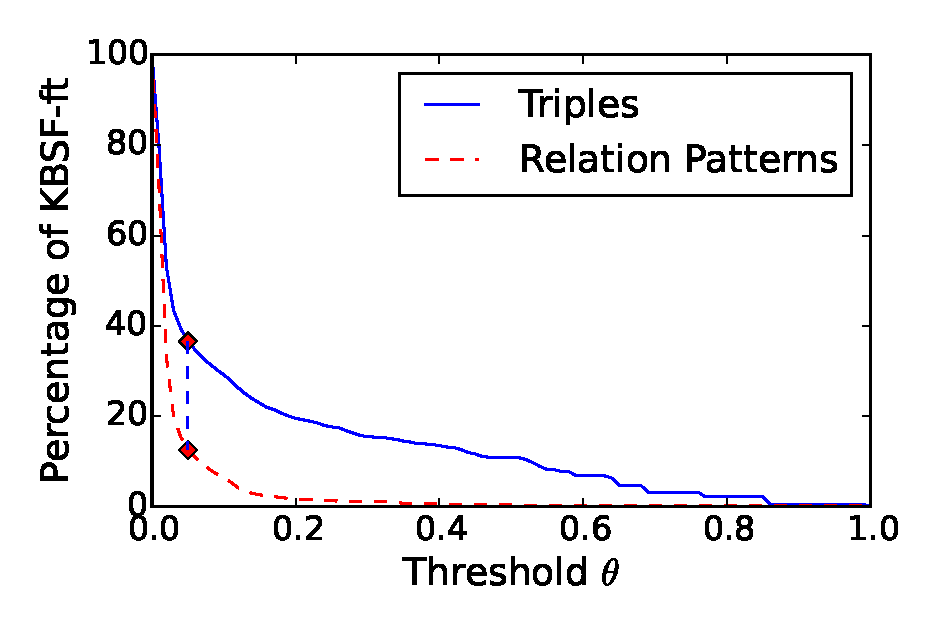
\includegraphics[width=6cm]{ch04_kbconstruction/pics/threshold.eps}}}
\caption{Percentage of triples and relation patterns from \textsc{KBSF}-ft that remain after pruning at different values of $\theta$. Maximum distance at $\theta=0.05$.}
\label{fig:kb:th}
\end{figure}

In addition, we created two baseline \textsc{KBs} for evaluation purposes. \textsc{KBSF}-co is a baseline which consists of simple entity co-occurrence. More specifically, if two entities are mentioned in the same sentence, an unlabelled triple that anchors them is added to the KB. In addition, \textsc{KBSF}-raw was created following the \textsc{RE} pipeline, but without applying the filtering process described in Section~\ref{sec:kb:method:re-filtering}. Finally, \textsc{KBSF}-rv constitutes the competitor \textsc{KB}, and is built as follows: After running \textsc{ReVerb} over the Songfacts dataset, we search coinciding relations, at both domain and range positions, that include entity mentions identified in our disambiguation step. These relations are included in KBSF-rv. Statistics about the five \textsc{KBs} are reported in Table \ref{tab:kbs}.

\begin{table*}[ht!]
\scriptsize
\centering
	\begin{tabular}{ | c | c | c | c | c | }
	\hline
	\textbf{KB} & \textbf{Entities} & \textbf{Triples} & \textbf{Relation Patterns} & \textbf{Cluster Patterns} \\
	\hline
	\textsc{KBSF}-ft & 20,744 & 32,055 & 20,438 & 14,481 \\
	\textsc{KBSF}-th & 10,977 & 11,720 & 2,484 & 828 \\
	\hline
	\textsc{KBSF}-co & 30,671 & 113,561 & --- & --- \\
	\textsc{KBSF}-raw & 29,280 & 71,517 & 47,089 & 32,712 \\
	\hline
	\textsc{KBSF}-rv & 9,255 & 7,532 & 2,830 & --- \\
	\hline
	\end{tabular}
	\caption{Statistics of all the learned \textsc{KBs}}
	\label{tab:kbs}
\end{table*}


\section{Experiments}
\label{sec:kb:experiments}

\subsection{Quality of Entity Linking}
\label{sec:kb:experiments:qualityentitylinking}

We mentioned in Section~\ref{sec:kb:method:entitylinking} the lacking of both music-specific \textsc{EL} tools as well as benchmarking datasets. For this reason, we performed a set of experiments to select the best-suited Entity Linking tool for the music domain, among some of the best known and reputed. Specifically, we perform evaluation experiments on \textsc{DBpedia} Spotlight, \textsc{TagMe} and \textsc{Babelfy}. 

%Let us briefly describe each of them: 

%\begin{itemize}
%    \item \textbf{Babelfy} \cite{Moroetal2014} A graph-based system for \textsc{EL} and Word Sense Disambiguation. It operates on the back of \textsc{BabelNet}, which serves as a reference sense inventory.
%    \item \textbf{Tagme} \cite{Ferraginaetal2010} An Entity Linking automatic annotator which matches terms with \textsc{Wikipedia} hyperlink texts and disambiguates them using both the in-link graph and the page datasets. It incorporates a context-aware pruning step.
%    \item \textbf{DBpedia Spotlight} \cite{Mendes2011} Automatically identifies entity mentions in free text, linking each match with its corresponding \textsc{DBpedia} URI.
%\end{itemize}

As of now, most \textsc{EL} systems \textit{speak their own language}, partially due to the fact that they perform entity disambiguation with different KBs as reference. Since their output is heterogeneous in format, performing a comparison between them is not straightforward. In order to evaluate the aforementioned EL systems, we used \textsc{ELVIS} (see Section~\ref{} in Chapter~\ref{}), an EL integration tool which provides a common output for different EL system.

In addition, we created a dataset of annotated musical entities and applied both quantitative and qualitative evaluations in order to verify which system performs better with musical entities, and is more suitable for our task.



\subsubsection{Evaluation Data}

We created an \textit{ad-hoc} gold standard dataset to evaluate the different EL systems, with the Songfacts dataset (Section~\ref{sec:kb:exp:dataset}) as our testbed. In this corpus, each document univocously refers to one single song. In addition, we have information about artist and song names at our disposal. We used this information to obtain the \textsc{MusicBrainz} ID for songs and artists. In \textsc{MusicBrainz}, artist and song items sometimes have information about their equivalent \textsc{Wikipedia} page. We leveraged this information, when available, to obtain their corresponding \textsc{DBpedia} URIs. Finally, we obtained a mapping with \textsc{DBpedia} of 7,691 songs and 3,670 artists. From the \textsc{DBpedia} resources of each song, we gathered their corresponding album name and URI, if available, obtaining information of about 2,092 albums. Then, for every document, we looked for exact string matches of the reported song, and its related album and artist names. Every detected entity is thus annotated with its \textsc{DBpedia} URI. At the end of this process, the newly created gold standard dataset contains 6,052 documents where 17,583 sentences are annotated with the following entities: 5,981 Song, 12,137 Artist and 1,722 Album entities. As mentioned in Section~\ref{sec:kb:method:entitylinking}, there are typical cases of ambiguity in musical entities where songs, artists and albums can potentially share the same name. Therefore, we manually corrected the entities detected in 212 documents where this kind of ambiguity was present.


\subsubsection{Entity Linking Evaluation}

\begin{table*}[ht!]
\scriptsize
\centering
	\begin{tabular}{ | c | c | c | c | c | c | c | c | c | c | }
	\hline
& \multicolumn{2}{|c|}{Album} & \multicolumn{2}{|c|}{Artist} & \multicolumn{2}{|c|}{Song} & \multicolumn{3}{|c|}{Macro Average}  \\
\hline
	& Prec & Rec & Prec & Rec & Prec & Rec & Prec & Rec & F-measure \\
	\hline
Babelfy & 0.93 & 0.28 & 0.98 & 0.55 & 0.96 & 0.31 & 0.96 & 0.38 & 0.54 \\
Tagme & 0.75 & 0.69 & 0.97 & 0.77 & 0.65 & 0.71 & 0.79 & 0.72 & \textbf{0.76} \\
Spotlight & 0.80 & 0.52 & 0.94 & 0.83 & 0.59 & 0.42 & 0.78 & 0.59 & 0.67 \\
\hline
	\end{tabular}
	\caption{Precision and recall of the Entity Linking Systems considered}
	\label{tbl:kb:res_categories}
\end{table*}

\begin{figure}[!htp]
\centerline{\framebox{
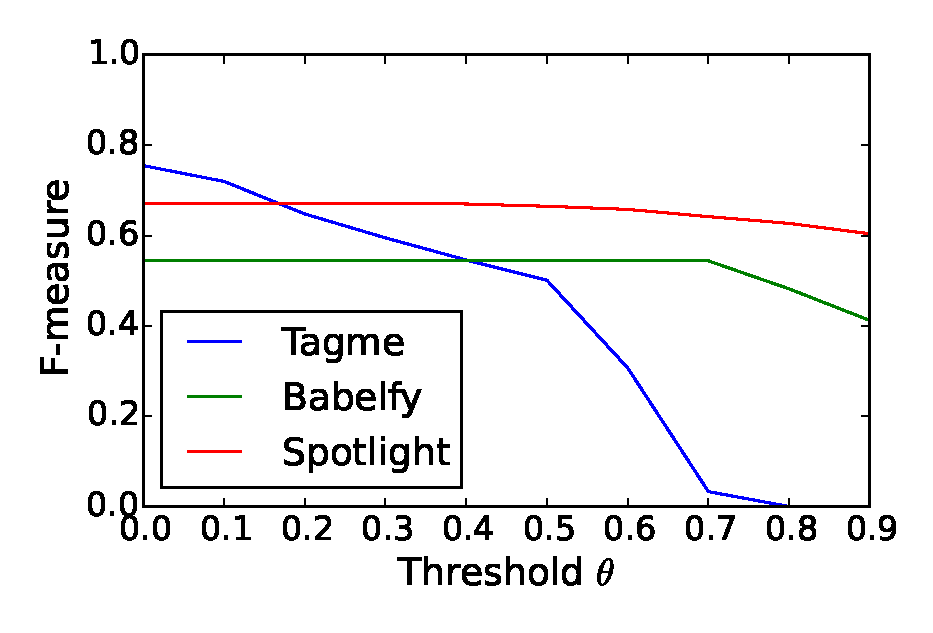
\includegraphics[width=6cm]{ch04_kbconstruction/pics/threshold_el.eps}}}
\caption{F-measure of the Entity Linking systems at different confidence thresholds}
\label{fig:kb:confidence_el}
\end{figure}

The three \textsc{EL} systems under review provide their own confidence measure. Hence, we evaluated their output filtering out the entities with a confidence measure below to a certain threshold $\theta$. We run the evaluation for different values of $\theta$, ranging from 0 to 0.9 in bins of 0.1. After evaluating on the gold dataset, the best results in terms of F-measure were obtained by all the systems at $\theta = 0$ (see Figure ~\ref{fig:kb:confidence_el}), which means that there is no need to apply any filtering process based on the \textsc{EL} system own confidence score. Detailed results on the run of every system at $\theta = 0$ are shown in Table~\ref{tbl:kb:res_categories}. We used macro-average Precision and Recall measures, i.e. we averaged their values from the three sets of entities.

We may conclude from these results that Babelfy is the system with highest Precision on musical entities. However, its recall is lower than the other systems under consideration, and specifically with respect to Tagme, which in turn, shows much lower precision. DBpedia Spotlight, on the other hand, achieves a similar precision score as Tagme, but with a slightly lower recall. 

This evaluation experiment is only focused on measuring the precision in the annotation of entities present in the gold standard. However, since all possible entities in a document may be not annotated, we also report on specific types of false positives which emerged during a qualitative inspection of classification results. For example, a frequent error that is not being evaluated concerns cases in which a text span not annotated in the ground truth is identified incorrectly as an entity by any system. Therefore, to complement the evaluation, we listed the most frequently identified entities by each system (see Table~\ref{tbl:kb:top_entities}). As we can see, Babelfy and Tagme are misidentifying common words as entities very frequently, whereas DBpedia Spotlight is not doing so. 
These errors may propagate to the rest of the \textsc{RE} pipeline, penalizing the accuracy of the final KB.
Although a filtering process could be applied to filter out misidentified entities by computing their tf-idf score in each document, we opted for using DBpedia Spotlight, as it has shown pretty good performance, its output does not require any further processing, and it is released as open source, which means that there are no limitations on the number of queries.

\begin{table*}[ht!]
\tiny
\centering
	\begin{tabular}{ | c | c | c | c |}
	\hline
System & Song & Album & Artist \\
	\hline
\multirow{5}{*}{Babelfy} & \textbf{Carey} & \textbf{Debut} & John\_Lennon \\
& \textbf{Stephen} & \textbf{Song\_For} & Eminem \\
& \textbf{Rap\_Song} & \textbf{Sort\_Of} & Paul\_McCartney \\
& \textbf{Singing\_This\_Song} & \textbf{First\_Song} & Bob\_Dylan \\
& \textbf{A\_Day\_in\_the\_Lif}e & \textbf{Debut\_Album} & Drake \\
	\hline
\multirow{5}{*}{Tagme} & \textbf{The\_Word} & \textbf{Up!} & John\_Lennon \\
& \textbf{The\_End} & \textbf{When\_We\_On} & \textbf{The\_Notorious\_B.I.G.} \\
& \textbf{If} & \textbf{U}p & \textbf{Do} \\
& \textbf{Once} & \textbf{Together} & Paul\_McCartney \\
& \textbf{For\_You} & \textbf{By\_the\_Way} & \textbf{Neil\_Young} \\
	\hline
\multirow{5}{*}{Spotlight} & Sexy\_Sadie &  The\_Wall & Madonna \\
& Helter\_Skelter & Let\_It\_Be & Eminem \\
& Cleveland\_Rocks & Born\_This\_Way & Rihanna \\
& Stairway\_to\_Heaven & Thriller & John\_Lennon \\
& Minnie\_the\_Moocher & Robyn & Britney\_Spears \\
	\hline
	\end{tabular}
	\caption{Top-5 most frequent entities by type and tool. Disambiguation errors appear in bold. }
	\label{tbl:kb:top_entities}
\end{table*}


\subsection{Quality of Relations}
\label{sec:kb:experiments:qualityofrelations}

\begin{figure}[t]
   \centering
    \begin{subfigure}[b]{0.49\textwidth}
        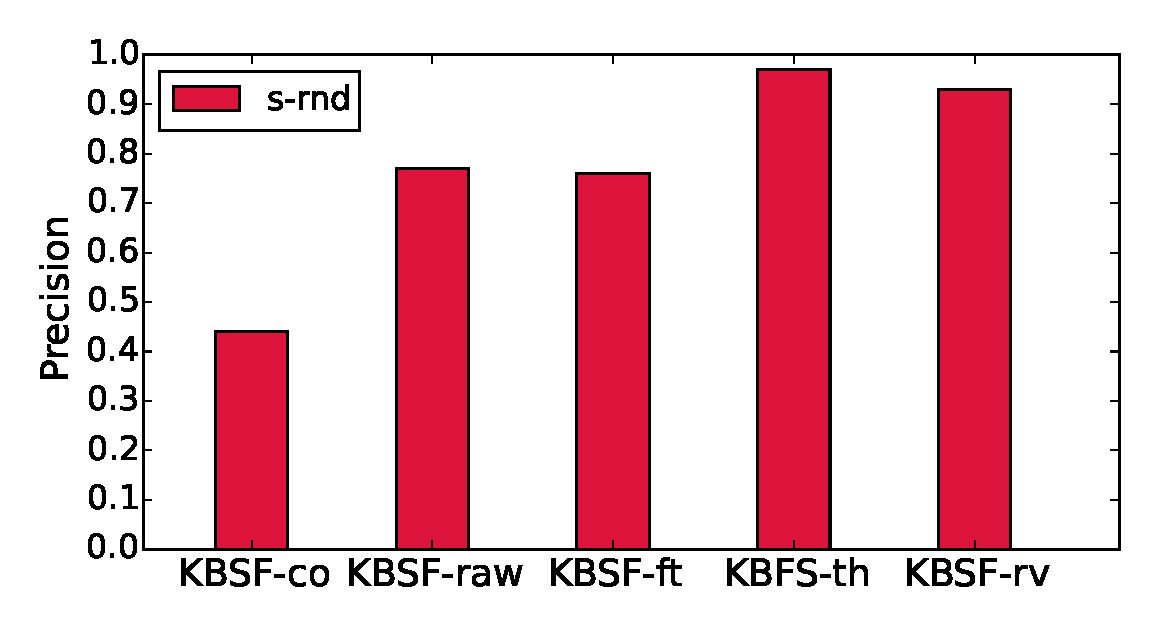
\includegraphics[width=\textwidth]{ch04_kbconstruction/pics/s-rnd100.eps}
        \caption{In sentence}
        \label{fig:kb:p_sentence}
    \end{subfigure}
    \begin{subfigure}[b]{0.49\textwidth}
        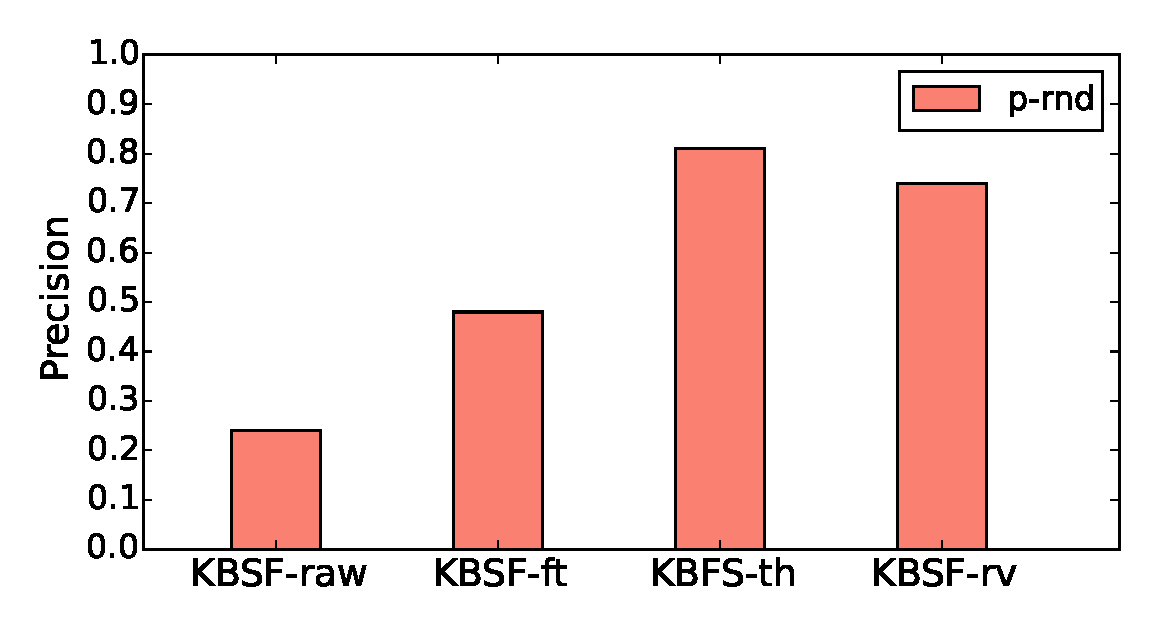
\includegraphics[width=\textwidth]{ch04_kbconstruction/pics/p-rnd100.eps}
        \caption{Relation patterns}
        \label{fig:kb:p_patterns}
    \end{subfigure}
    \begin{subfigure}[b]{0.49\textwidth}
        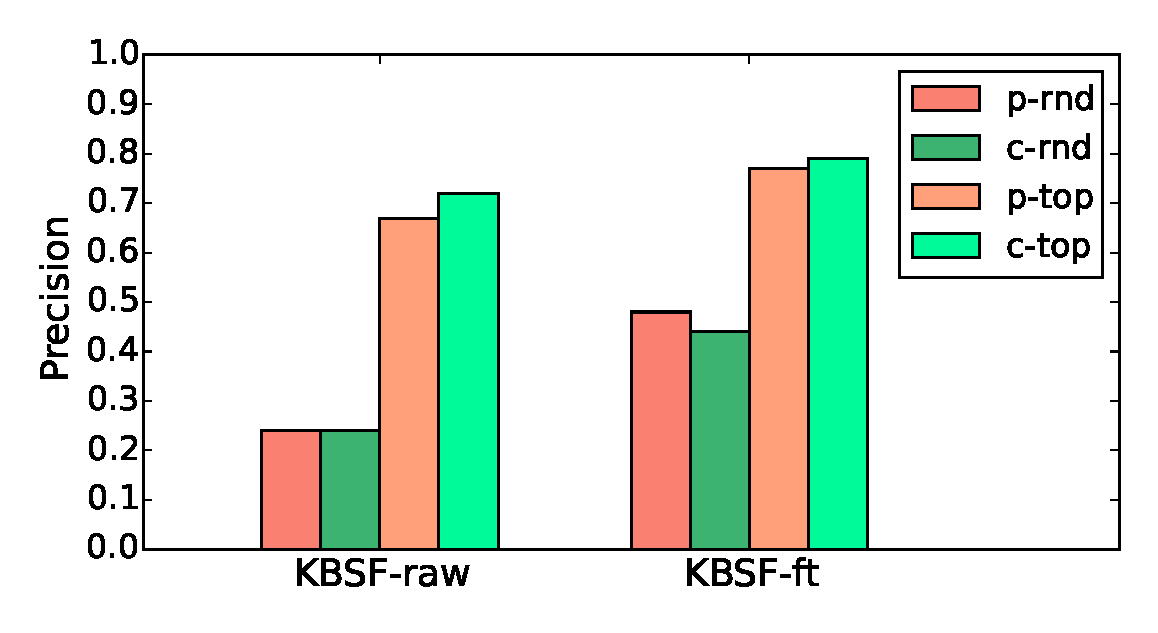
\includegraphics[width=\textwidth]{ch04_kbconstruction/pics/eval_p_c.eps}
        \caption{Patterns and clusters}
        \label{fig:kb:p_clusters}
    \end{subfigure}
    \caption{Precision of relations at sentence (\textit{s}), relation pattern (\textit{p}) and cluster pattern (\textit{c}) levels in top (\textit{top}) and random (\textit{rnd}) samples of relations}\label{fig:kb:eval_relations}
\end{figure}

\textsc{RE} evaluation is not trivial, as semantic relations between entities may vary in terms of correctness over time. Also, correct relations may be linguistically flawed, i.e. not fluent. Previous approaches assessed automatically extracted relations in terms of correctness according to human judgement \cite{Fader2011,Mausam2012}. Additionally, a finer grained analysis is carried out in \cite{Bankoetal2007}, adding a prior step in which relations are judged as being \textit{concrete} or \textit{abstract}.

In this chapter, we made use of extensive human input and asked two experts in Computational Linguistics to evaluate the \textit{top 100} scoring relations as yielded by our weighting policy (Section \ref{sec:kb:method:scoring}), as well as a random sample of 100 relations. This was done for all the \textsc{KBs} produced by our pipeline and for \textsc{KBSF}-rv. Cohen's kappa coefficient ranged from 0.60 to 0.81, which is generally considered as \textit{substantial} agreement.


In Figures \ref{fig:kb:p_sentence} and \ref{fig:kb:p_patterns}, where we compare random samples from each \textsc{KB}, we observe a gradual improvement of the quality of relations as the different modules of our implementation are incorporated. The difference between these figures is that in the former, a relation is deemed correct if it has extracted a relation \textit{expressed in the original sentence}, whereas the latter figure reports numbers on whether the extracted relation pattern was correct, i.e. if it \textit{meant} the same as it was intended in the source sentence. We may infer from these results that co-occurrence between entities does not guarantee an explicit relation, whereas the presence of a path between two entities over a sentence dependency tree, without any other entity mention in between, generally suggests a monsemous and unambiguous relation.

It is remarkable how well \textsc{ReVerb} performs (Figure \ref{fig:kb:p_patterns}), only being surpassed by the \textsc{KB} resulting from the complete implementation described in this chapter. We note that the good results of the \textsc{ReVerb} extractor are also due to the semantic processing of our system, which is forcing \textsc{ReVerb} to select good candidates as relation arguments. Recall that the difference between \textsc{KBSF}-ft and \textsc{KBSC}-th is the inclusion of the \textit{scoring} module, and the increase in Precision confirms that incorporating \textit{statistical evidence contributes to better relations}.

This is further confirmed in the results showcased in Figure \ref{fig:kb:p_clusters}, where we provide a comparison between top 100 relations according to our ranking policy against a random sample. Note that \textit{in all \textsc{KBs}, highly scoring relations are more often marked as correct}, which constitutes additional support for the contribution of the scoring module. Together with the quality of the relation pattern, this figure shows the quality of the cluster pattern associated with the evaluated relations. We observe that cluster patterns inferred in our clustering module have similar quality than relation patterns in the random sample, and slightly better in the top 100 sample. This result implies that the scoring module is rewarding good clusters.

\subsection{Coverage of the Extracted Knowledge Base}
\label{sec:kb:experiments:coverage}

With this experiment, we aim to compare the coverage of music relations in our \textsc{KBs} with respect to other resources with human intervention, such as \textsc{DBpedia}, \textsc{MusicBrainz}, and with fully automatic resources. For the latter, we considered \textsc{DefIE} as our closest competitor due to several methodological similarities (dependency parsing, \textsc{EL} and \textsc{RE} over shortest paths). 

We selected all triples in \textsc{KBSF}-th whose domain and range entities could be mapped to both \textsc{DBpedia} and \textsc{MusicBrainz}. As our extracted \textsc{KB} has only MusicBrainz ID of entities of types MusicalArtist and Song, the set of triples to evaluate is restricted to relations between them. Since entities in \textsc{DefIE} are disambiguated against \textsc{BabelNet} ids, we mapped all \textsc{DBpedia} uris to their corresponding \textsc{BabelNet} id, which yielded a subset of 3,633 triples. From here, we selected all possible domain-range entity pairs, and retrieved from the other \textsc{KBs} all triples with the same pairs, and counted them.
The procedure to do so on \textsc{DBpedia} was via SPARQL queries.
We discarded triples with predicate \textit{wikiPageWikiLink}, as this predicate means an unlabeled relation. However, the mapping with \textsc{MusicBrainz} was not trivial. \textsc{MusicBrainz} is not a \textsc{KB} of triples, but a relational database. Entities are stored in tables, and relations between entities are represented in a set of tables of relations, having one table for each possible relation. The entities in the studied set of triples were only of type MusicalArtist and Song. However, an entity of type Song in \textsc{KBSF}-th can be related to either a Recording or a Work entity in \textsc{MusicBrainz} (see Section~\ref{sec:kb:method:typefiltering}). Therefore, for the analysis of relations involving a Song entity, we obtained the equivalent Recording and Work \textsc{MusicBrainz} entities, and looked up relations where any of them where present.

Mapping results are shown in Table~\ref{tbl:kb:coverage}. Let us highlight the fact that most semantic relations encoded in \textsc{KBSF}-th are novel, as they were not found in any of the other resources we compared against. In the overlapping cases, most of the times the relation labels were semantically equivalent, and often the relation label of \textsc{KBSF}-th triples was more specific than the ones retrieved from other \textsc{KB}s (e.g. \textit{frontman} and \textit{member of})

\begin{table*}[ht!]
\scriptsize
\centering
	\begin{tabular}{ | c | c | c | c | c |}
	\hline
	& KBSF-th & MusicBrainz & DBpedia & DefIE \\
	\hline
	Relation instances & 3,633 & 1,535 & 1,240 & 456 \\
%	Relation patterns & 746 & 24 & 32 &  \\
	\hline
	\end{tabular}
	\caption{Number of triples with labeled relations in the different KBs for the same set of domain-range entity pairs}
	\label{tbl:kb:coverage}
\end{table*}


\subsection{Interpretation of Music Recommendations}
\label{sec:kb:experiments:recommendation}

The main aim of this experiment is to evaluate the suitability of \textsc{KBSF}-th to explain relations between songs, and study their impact on user's experience in music recommendation. 
Since our aim is not to measure the performance of a recommender system, we implemented a baseline recommender approach. Recommendations are based on the concept of song similarity, which exploits the graph-based structure of our \textsc{KB}. Maximal common subgraph score is computed between the item neighborhood graphs of every song. This methodology for entity similarity is fully described in Section~\ref{sec:similarity:method:sim:mcs} of Chapter~\ref{sec:similarity}. Once the similarity scores are computed, similar songs for every song are ranked based on it.


We designed the experiment as an online survey, where the participant is first asked to select 5 songs from different artists of his/her choice. From each selected song, the system randomly selects 3 recommendations among the list of its top-10 most similar songs. One of them is shown together with an explanation in natural language (the source text), another with an explanation based on relation patterns, and finally the third one appears without explanation.
Participants can listen to all songs with an embedded player. After listening to the recommendation and reading the explanation attached to it, participants were asked to rate each recommendation from 1 to 5 (1 being worst), and to mention whether they were familiar or not with the recommended songs (see Figure~\ref{fig:kb:recommender}).


The experiment involved 35 participants, 28 males and 7 females, ranging from 26 to 38 years old and with different musical background and listening habits. Most of the participants said that they had previous experience with recommendation systems. 
A total of 525 answers (corresponding to individual song recommendations) were collected. In 38\% of the cases, the user was familiar with the recommended songs.

The average rating of recommendations with natural language explanations is slightly higher (3.20$\pm$1.29) than recommendations without explanations (3.08$\pm$1.35), or with explanations based on relation labels (3.04$\pm$1.34). In addition, for musically educated individuals, recommendations of unfamiliar songs, whether accompanied with or without explanations, have similar average rating (2.87 and 2.95 respectively). However, for untrained users, recommendations with explanations have a remarkable higher average rating (2.93) than without them (2.36). Thus, we can infer that the introduction of explanations in recommender systems improves the user experience of musically untrained subjects when discovering songs.

We also asked the subjects to select among a set of adjectives those that better described the recommendation experience. The general trend was to rate positively the experiment. Most users rated the experience as \textit{enjoyable} (40\%), followed by \textit{useful} (31\%) and enriching (29\%). Negativity was much lower in general, with \textit{confusing} being the most voted (17\%), followed by \textit{complicated} and \textit{too geeky} (8\% in both cases). This suggests that the introduction of explanations generated from our \textsc{MKB} in the recommendations was in general a satisfactory experience to users.


\begin{figure}[!htp]
\centerline{
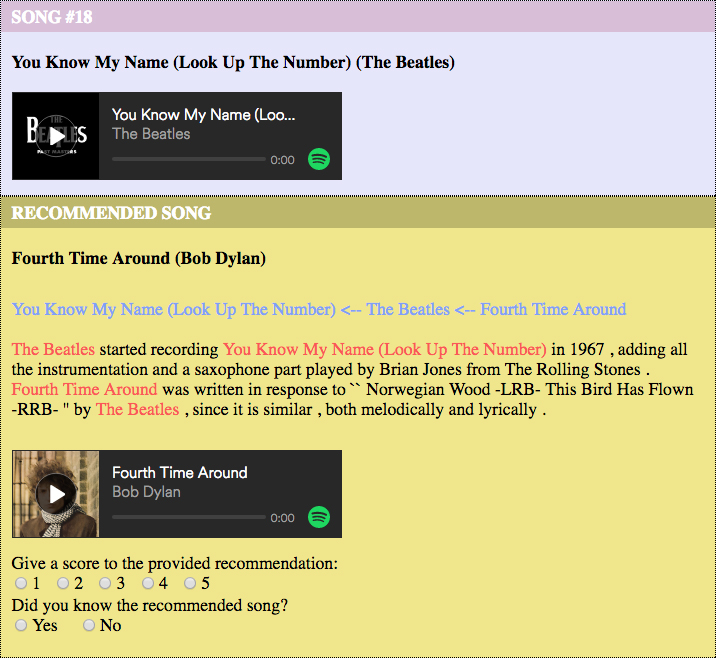
\includegraphics[width=0.6\textwidth]{ch04_kbconstruction/pics/recommender.jpg}}
\caption{User interface for the music recommendation experiment.}
\label{fig:kb:recommender}
\end{figure}


\section{Conclusion}\label{sec:kb:conclusions}

We have presented an NLP pipeline that learns a Knowledge Base in the music domain taking raw text collections as input. It combines methods easily applicable to a general purpose application with domain-specific heuristics which are designed to exploit particularities of the domain.

The result of applying our approach over a dataset of stories about songs is a new Music Knowledge Base, which encodes semantic relations among musical entities. Our method relies on the syntactic structure (defined via dependency parsing) of sentences and the use and adaptation of music-specific heuristics for both \textsc{EL} and \textsc{RE}. In addition, we include modules for semantic clustering and pattern scoring, aimed at the efficient removal of noisy relations. Our modular evaluation shows that our \textsc{RE} module is able to capture a highly precise and compact set of weighted triples, and demonstrates the positive impact of the novel scoring metric we introduced. Moreover, we have shown that a high percentage of the knowledge encoded in our \textsc{MKB} is not present in other \textsc{KB}s, both general and domain-specific. Finally, regarding extrinsic evaluation, the experiment on recommendation interpretation confirms that explanations based on the learned \textsc{KB} are positively regarded by the users.

%In the following chapter, we propose a method 

%We have identified several promising avenues for future work. For instance, we would like to extend our experiments to other music datasets of varied registers (e.g. social networks, magazines, encyclopedias), in order to fully understand the core differences between this domain and standard language. This should give an approximate idea of whether we need specific tools in certain specific NLP tasks. For instance, it seems reasonable to envision a music \textsc{EL} tool that is able to cope better with certain particularities of the domain.
%In addition, the development of new methodologies in Music Information Retrieval that exploit \textsc{MKB}s is still an open area of research.
